\section{Schlussfolgerungen}
\label{sec:schlussfolgerungen}

In dieser Arbeit haben wir versucht Techniken und Methoden aufzuzeigen welche
es ermöglichen Entwicklungszyklen drastisch zu verkürzen. Ausgehend von einem
jährlichen Entwicklungszyklus wurden schrittweise Maßnahmen vorgestellt um die
Kadenz der Releases zunächst auf vierteljährlich, monatlich, wöchentlich und
zu guter Letzt auf täglich umzustellen. Dabei wurden nicht immer nur neue
Praktiken hinzugefügt sondern, sofern erforderlich auch bestehende als
schlecht aufgezeigt und für obsolet ja sogar hinderlich (Ballast) erklärt.
Eine Übericht aller vorgestellten Techniken und Methoden ist in
Tabelle~\ref{tab:uebersicht} auf Seite~\pageref{tab:uebersicht} aufgelistet.


\begin{table}[htbp]
    \centering
        \caption{Übersicht über die Best Practices}
        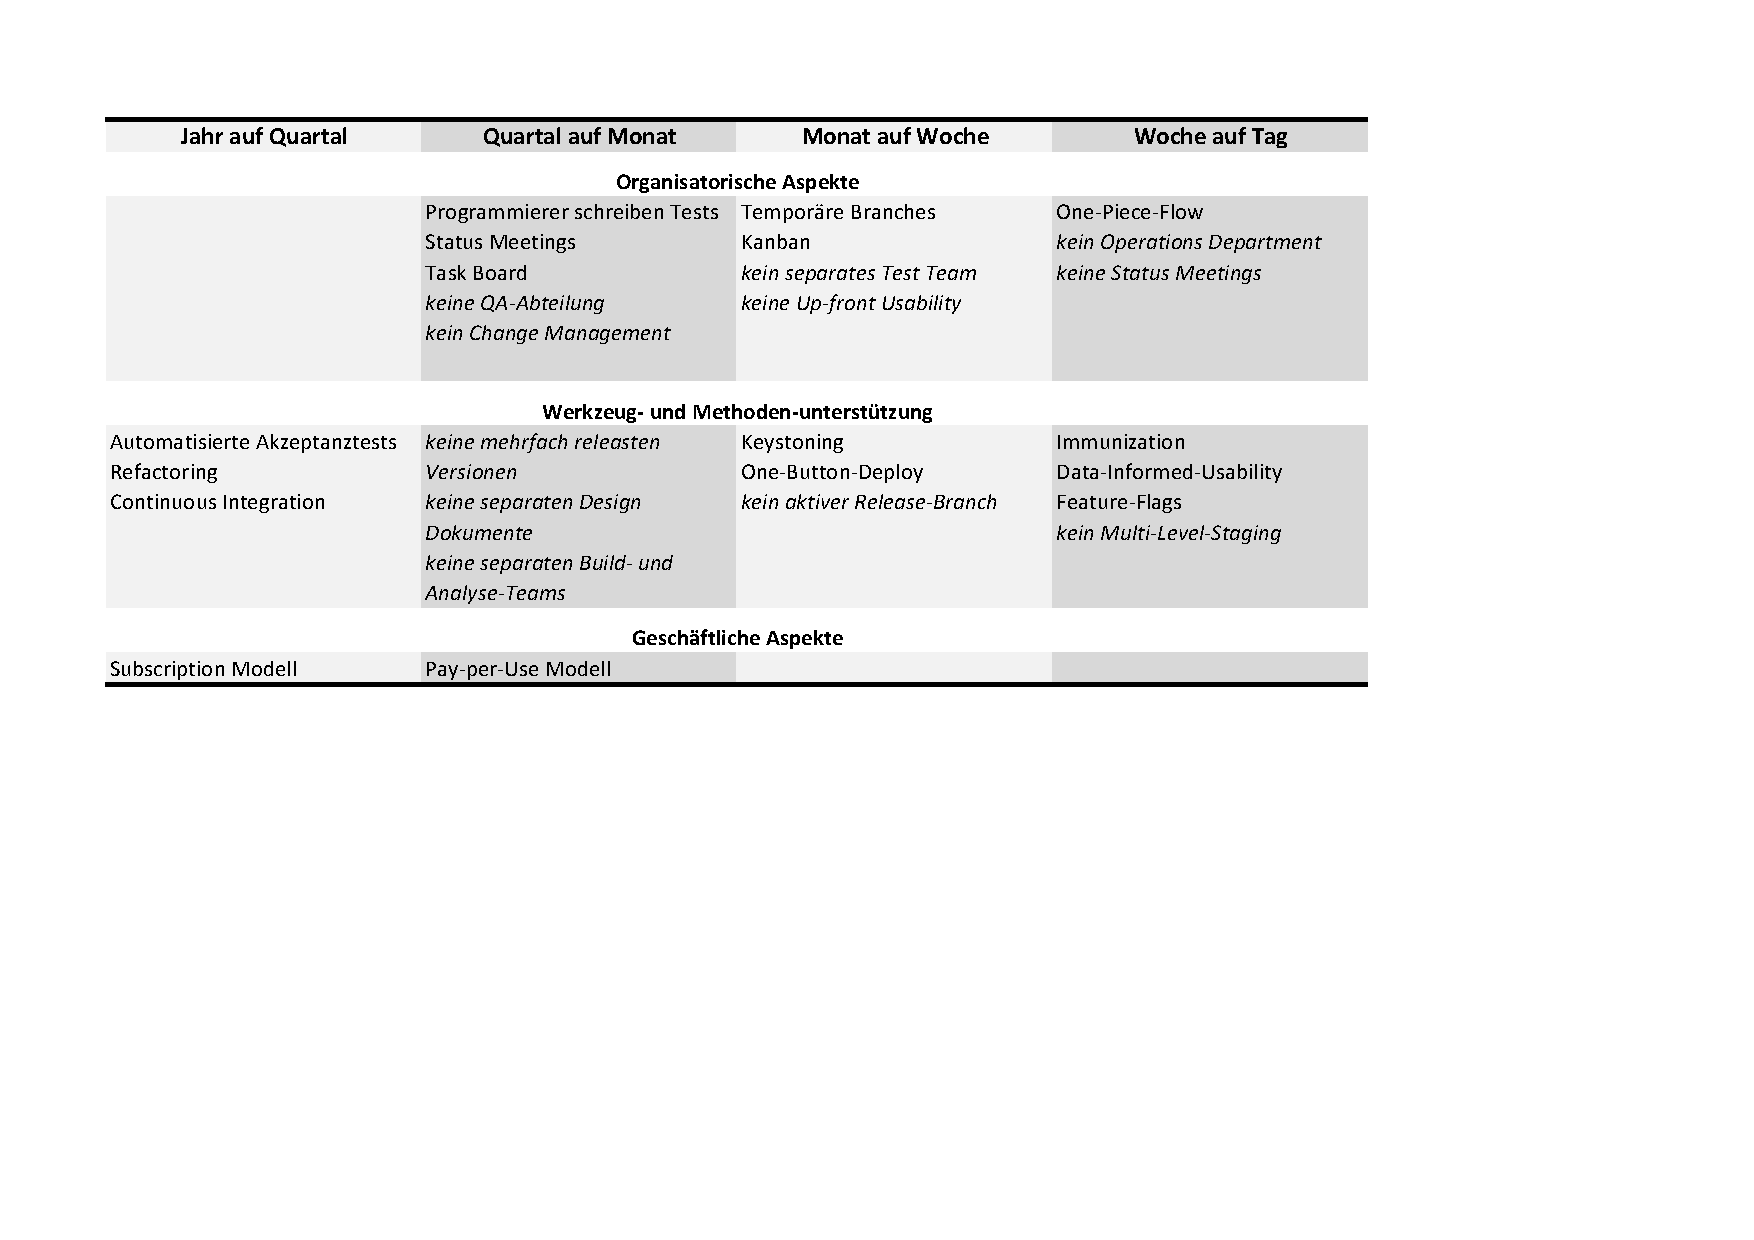
\includegraphics[trim = 50bp 265bp 185bp 56bp, clip, width=1.00\textwidth]{uebersicht}
    \label{tab:uebersicht}
\end{table}

\begin{quote}
\zitat{Does this mean we're never going to introduce bugs to our live site? Of
course not - but we're going to keep the number of bugs to hit the live site
to a minimum, and we've made it easy and fast to get bug fixes live as
well.}~\cite{digg4}
\end{quote}
